% !TEX program = xelatex
% !BIB program = biber
\documentclass[headinclude]{scrbook}
\usepackage{classicthesis}
%\usepackage[left=1.25in,right=1.25in,top=1in,bottom=1in]{geometry}
\usepackage{graphicx}
\usepackage{subcaption}
\usepackage[binary-units=true]{siunitx}
\usepackage{float}
\usepackage{pgfplots}
\usepackage{listings}
\lstset{frame=tb,
basicstyle=\ttfamily,
language=Lisp}

\pgfplotsset{compat=1.14}

\tolerance=1000

\newcommand\mytodo[1]{[[\textcolor{red}{#1}]]}

\usepackage{microtype}
%\microtypesetup{protrusion=false,expansion=true,auto=true,tracking=true}
\hyphenation{block-chain}
\hyphenation{block-chains}
\hyphenation{Byz-an-tine}
\hyphenation{vir-tual-chain vir-tual-chains}
\hyphenation{crypto-curren-cy}


\usepackage{fontspec}
\setmainfont[BoldFont={* Semibold}]{Linux Libertine O}
%\linespread{1.1}
\setmonofont[Scale=MatchLowercase]{Latin Modern Mono}
\setsansfont[Scale=MatchLowercase]{Inter}

%\usepackage{libertine}

%\usepackage[sc]{mathpazo}
%\linespread{1.05}
%\usepackage{eulervm}

\graphicspath{{assets/}}

\usepackage{hyperref}
\hypersetup{
    colorlinks,
    citecolor=black,
    filecolor=black,
    linkcolor=black,
    urlcolor=black
}

% BibTeX
\usepackage[backend=biber]{biblatex}
%\renewbibmacro{in:}{}
\addbibresource{whitepaper.bib}


\begin{document}
%\raggedbottom
\title{Themelio: a layer-0 public blockchain}
\author{Themelio Labs}
\date{\today}
\maketitle

%\begin{abstract}

%\end{abstract}

\tableofcontents


\chapter{Introduction and motivation}

\section{The ``blockchain revolution'': expectations vs reality}

\subsection{The promise of blockchains}

Trust on the Internet is a rare commodity. Participants are often anonymous, and communication is inherently insecure. Everybody is at most a few hundred milliseconds away from potential attackers.

Generally, to trust someone on the internet you either know them in real life or depend on trusted third party intermediaries. However, real-world knowledge is extremely unlikely to exist on the Internet, and intermediaries, such as certificate authorities, lookup servers, and notaries are almost always centralized institutions. Unfortunately, central points of trust are often single points of failure. Compromised root CAs lead to catastrophic meltdowns of the basic cryptography of the encrypted Web \cite{prins2011diginotar}. Poisoned DNS servers enable defacings of high-profile websites. Hacked update servers can instantly distribute malware to enormous numbers of unsuspecting computers, crippling critical systems \cite{richardson2017ransomware}.

Moreover, centralized control of the ``commanding heights'' of our modern interconnected society lends a disproportionate amount of power to a small oligarchy of service providers. This enables a wide range of abuse, with devastating real-world consequences. For instance, centralized social media platforms insidiously manipulate and censor user communication \cite{sunstein2018republic}. Governments build Orwellian surveillance systems like the prototype Chinese ``social credit'' system \cite{wang11china} by aggregating massive amounts of data from centralized sources.

Public blockchains like Bitcoin \cite{nakamoto2008bitcoin} and Ethereum \cite{wood2014ethereum} are unforgeable, append-only ledgers accessible to all. They provide secure, transparent, and permanent records of transactions while being completely decentralized. Instead of relying on unaccountable centralized entities, applications such as public key infrastructures, document timestamping services, and electronic money can now use this shared ledger to guarantee security. Blockchains promise a revolution to end reliance on dangerously fragile central trusted entities.


\subsection{Where are all the blockchain apps?}

Despite all the hype of a blockchain revolution, almost no production systems use public blockchains. Naming even a \emph{single} user-facing application using a public blockchain is astonishingly difficult --- exempting, of course, cryptocurrency trading apps, blockchain viewers, and such. Why?

We believe it's simply because \emph{public blockchains aren't good enough}. First of all, Nakamoto consensus, the very innovation that gives public blockchains their robust decentralized consensus, saddles users with onerous costs. Take Bitcoin as an example: users must synchronize and store the blockchain's entire transaction history --- hundreds of gigabytes and growing --- and, when the network is even a little untrusted, wait hours for transactions to become irreversible.

Furthermore, public blockchains can be quite unreliable. Wildly fluctuating cryptocurrency prices create unnecessary currency risk, congestion leads to spikes in transaction fees, and network problems cause long delays. None of these flaws are acceptable in production systems. Finally, public blockchains by nature require unanimous agreement on the blockchain protocol. Therefore, protocol upgrades are almost always disruptive and contentious --- every little change can shake the whole blockchain ecosystem. Nobody wants to build applications on foundations that threaten their products' stability with every update.

Unsurprisingly, blockchains have failed to truly revolutionize industry. Instead, their  impact is mostly limited to inspiring a breed of centralized databases with the catchy label of ``private blockchains''. Although private blockchains, like those based on Hyperledger Fabric \cite{cachin2016architecture}, use append-only distributed ledgers similar to those of public blockchains, they're generally deployed within an environment isolated from public access, such as across a corporate WAN or even inside a single datacenter. Enterprise applications, such as supply-chain tracking or processing business payments, have an especially strong tendency towards using private blockchains. ``Blockchain for business'' is almost a synonym to a blockchain within a private, controlled environment. Unlike their public counterparts, private blockchains promise performance and reliability comparable with traditional databases. For this reason, private blockchains have been adopted by a wide variety of production systems, ranging from the SecureKey identity service \cite{securekey} to Estonian government systems \cite{estonia}.

However, private blockchains by definition give up much of the security, transparency, and decentralization of public blockchains. Most proposed deployments, such as those within a single datacenter, almost entirely abandon the promised paradigm shift towards decentralization. Private blockchains' pursuit of maximal usability has rendered them useless in bringing about a more decentralized Internet.

\section{A better blockchain?}

\subsection{Existing attempts}

Of course, many projects do attempt to build better blockchains than currently existing ones. One fairly obvious class of ideas is simply compromising between private and public blockchains to get the best of both. ``Consortium'' blockchains --- blockchains where participation is limited to a small number of trusted partners --- are a good example. For example, banks may partner to create a consortium blockchain for an interbank settlement cryptocurrency. Consortium blockchains may also support access, though not participation in the consensus protocol, from the public. Some blockchains, like EOS, even elect the consortium from the wider public.

Limiting the number of blockchain consensus participants typically improves performance and reliability for the same reasons private blockchains are better in these aspects: the data needs to be replicated much fewer times. Unfortunately, these ``hybrid'' blockchains retain most of the problems of either public or private blockchains. Those that deliver reliable performance and agile updates end up with the poor security and inadequate decentralization of private blockchains. Other more secure ones inherit the problematic performance and inflexibility of public blockchains. Ultimately, retaining decentralized trust requires wide-scale consensus, while reducing the overhead of consensus necessarily translates into less security and neutrality.

Another approach is abandoning the model of a unified, trustless append-only log. This includes ``sharded'' designs for blockchains, such as those planned for Ethereum, and non-blockchain ledgers like Ripple and Hashgraph. Though forgoing the requirement for a universally replicated log eliminates most scalability challenges, it introduces much greater complexity in both implementation and application interfaces. This only exacerbates the already daunting difficulty in developing applications on blockchains. In fact, none of these ``unconventional'' distributed ledgers have achieved much production success. After all, distributed consensus protocols have existed for decades. It is precisely the simple yet expressive abstraction of a linear blockchain that has fascinated the world.


\subsection{The crux: a layering problem}

Our discussion on existing blockchains leads to the conclusion that there is yet to be a public blockchain that can realize the paradigm shift promised by the ``blockchain revolution''. Performance issues still plague public blockchains: classical problems such as replication costs persist, while new difficulties related to advanced features like smart contracts emerge. Security and decentralization remain difficult, with trustworthy safety available only at the cost of debilitatingly poor performance.

However, the biggest obstacle keeping public blockchains from widespread adoption is probably not technical deficiency, but rather design philosophy. More specifically, \textit{blockchains are on the wrong layer} in application protocol stacks. Current blockchain designs typically fall into two camps:

\begin{itemize}
    \item \textbf{Single-purpose blockchains} are optimized for one particular application. They often have adequate usability and performance at the expense of adaptability to diverse usages. Examples include Bitcoin Cash (higher throughput bitcoin), Filecoin (incentivized peer-to-peer content distribution), and Zcash (untraceable payments).
    \item \textbf{``Swiss army knife'' blockchains} attempt to provide the full set of features needed to implement decentralized applications, typically through Turing-complete ``smart contracts''. Ethereum is the archetypal Swiss army knife blockchain; newer examples include EOS and Tezos.
\end{itemize}

In our opinion, neither of these paradigms work. This is a surprising assertion --- a single-purpose blockchain obviously cannot support a global ecosystem of decentralized apps, but what's wrong with blockchains like Ethereum that are based on generalized smart contracts?

In short, \textit{smart contracts are too smart}. Yes, smart contracts allow easy deployment of applications directly on top of the blockchain --- a new cryptocurrency can be implemented on Ethereum in a few dozen lines of code. However, such a direct interface between application and blockchain inevitably results in conflict between ever-changing application requirements and ideally immutable blockchain protocols.

Take Ethereum as an example. Ethererum aspires to be a ``simple'' platform with ``no features'' based on a simple smart contract language (EVM)  that ``any average programmer can implement'' \cite{buterin2014ethereum}. Since its inception, however, Ethereum has accrued feature after feature, while EVM's list of opcodes has grown longer and longer. To implement these changes, consensus-breaking ``hard forks'' have repeatedly occurred. Today, Ethereum is an extremely complex system with a reference implementation of almost a million lines of code \footnote{More precisely, 828,000 lines of code, mostly in Go, are present in the Geth implementation as of October 2018. On the other hand, \texttt{btcd}, a Go implementation of Bitcoin, contains merely 94,000 lines.}. Such complexity and mutability, we believe, has no place in the foundational root of trust blockchains are supposed to provide.

In summary, blockchains today are either on the application layer, or the layer immediately underneath it. Both of these layers are far too complex and change way too fast to be in the base protocol of a blockchain. Blockchains should be simple and immutable.

Let's switch gears from blockchains and take inspiration from the technology underpinning most of modern telecommunication: the Internet Protocol (IP). IP gets packets on a best-effort basis from point A to point B, and nothing more. It is precisely this simplicity that allows it to support the dazzling variety of Internet applications today with practically no changes since the IPv4 specification's publication in 1981.

Unreliable datagrams don't make a developer-friendly interface, but they do provide a firm foundation for ever-changing application protocol stacks. IP is a great illustration of a successful foundational technology. Such protocols are often too simple to support rich applications without intervening protocol stacks, but they are easy to conceptualize, simple to implement, and brutally robust.

We've designed Themelio, a new public blockchain, according to this vision of a simple and stable base protocol. We focus on providing a basic and robust decentralized root of trust, with very good performance and security. Many layers of abstraction may separate applications from Themelio, but this allows it to change very little as usages evolve. Themelio is a neutral, immutable fabric that can truly support a vibrant ecosystem of decentralized-trust applications.


\chapter{Themelio's design}

In our introduction, we laid out our vision for Themelio. Instead of a specific decentralized application or a ``Swiss army knife'' runtime environment, Themelio provides a \emph{universal decentralized root of trust}. We want Themelio to sit at the bottom of diverse and evolving protocol stacks, providing a foundation of decentralized trust and consensus --- but not much else.

But how are we to build such a blockchain? We combine an elegant, time-tested application interface --- a ``coin-based'' transaction graph like that of Bitcoin --- with numerous innovations under the hood. Consensus, based on proof of stake, is immediate, scalable, and highly secure. Cryptocurrency is issued in a completely decentralized manner, yet remains immune to bubbles that destabilize the exchange rate. A simple yet expressive scripting language allows developing advanced decentralized apps without the problems associated with stateful smart contracts. These are some of the many features we use to maximize robustness and performance.

\section{Design goals}

Before we take a dive into the details of Themelio's architecture, let's first examine what we want to accomplish, and what we don't.

\subsection{Goals}

Our overarching goal of being a foundational root of trust leads us to design Themelio according to these principles:

\begin{enumerate}
    \item \textbf{Simple abstractions}: Themelio should present simple, ``non-leaking'' abstractions. Programmers without much experience with blockchains should be able to easily understand the features and behavior of the Themelio blockchain. We try our very best to avoid forcing users to consider subtle edge cases. For example, we must avoid many blockchains' unintuitive behavior in the presence of network latency (``confirmations'', forks, reorganizations).
    \item \textbf{Stable protocol}: An initial period of rapid evolution is inevitable. But once mature, Themelio's internals should change as little as possible. Protocol stability avoids dangerous and messy consensus-breaking updates. Even though many blockchains envision constant protocol evolution, this introduces difficult out-of-band coordination problems --- otherwise known as politics.  This can easily lead to de-facto centralization, contentious forks, and subversion by special interests. In Themelio, consensus-breaking changes will be made only in exceptional, non-controversial circumstances, such as to fix critical security vulnerabilities.
    \item \textbf{Currency stability}: Themelio's cryptocurrency, the mel, is designed to have very low price volatility. It avoids large price increases, even with spikes in demand. The mel is designed to be a good unit of account and store of value, not a speculative asset exciting to ``HODL''.
    \item \textbf{High performance}: Themelio's performance must be much higher than existing public blockchains. This means both high transaction throughput and scalability in the number of fully secure clients. Decentralized apps with debilitatingly poor performance cannot take over the world.
    \item \textbf{Application neutrality}: Themelio should not attempt to prevent or censor any categories of applications. It does not have an ``intended use''.
    \item \textbf{Robust decentralization}: The ideal public blockchain must simulate a universally trusted intermediary --- decentralization is a must. Themelio is designed to decentralize trust across as large a population of stakeholders as possible. No unaccountable third parties, including network operators, should be able to subvert its security guarantees.
\end{enumerate}

\section{A robust transaction model}

We start with a conceptual exploration of Themelio's high-level transaction model: the abstractions on the blockchain that applications interact with.

\subsection{Coin-based transactions}

Themelio's basic transaction model belongs to a family usually known as ``UTXO-based'' or ``coin-based'' models. This is the oldest family of blockchain models, including first-generation blockchains like Bitcoin and Litecoin. In a coin-based model, the blockchain can be understood as a grow-only directed acyclic graph (DAG) of \emph{transactions}. Every transaction on the blockchain takes as input and spends one or more \emph{unspent transaction outputs (UTXOs)} of previous transactions, which are informally known as \textit{coins}. It then produces as output one or more coins that can be spent as input by subsequent transactions.

Every coin represents a given amount of cryptocurrency, known as its \emph{value}, and it includes an \emph{unlock constraint} that specifies what sort of transaction can spend the coin. Each coin can only be spent once. Excepting transactions that ``mine'' more currency, the sum of the values of all the coins spent by a transaction must equal the sum of the values of all the coins created by it.

Let's illustrate how coin-based transactions work with a simple example. Assume there are 5 coins identified as $B_1,\dots,B_{5}$, each worth \$1, and each having an unlock constraint specifying ``any transaction that spends me must have Bob's signature''. Informally, we say that Bob owns 5 coins, each one worth \$1. Bob ``owning'' a coin simply means Bob knowing how to satisfy the coin's unlock constraint.

Now, assume that Bob wants to send his friend Alice \$2.5. He creates a new transaction spending $B_1,B_2,B_3$ as input, with two outputs:
\begin{itemize}
    \item $A_1$ with value \$2.5 and a constraint requiring Alice's signature.
    \item $B_6$ with value \$0.5 and a constraint requiring Bob's signature.
\end{itemize}
and informs Alice about $A_1$. Bob now ``owns'' $B_4,B_5,B_6$ with a total value of \$2.5, and Alice owns $A_1$ with a total value of \$2.5, just as we wanted. Note that Bob had to give himself a new coin for the transaction to balance; this new coin is known as a \emph{change output}. Figure \ref{fig:utxo} from bitcoin.org shows a complex series of interdependent coin-based transactions.

\begin{figure}
    \centering \includegraphics[width=\linewidth]{utxo.pdf}
    \caption{Coin-based transactions in Bitcoin}
    \label{fig:utxo}
\end{figure}


Transactions are batched into an ever-growing series of \emph{blocks}, each one containing transactions settled in a particular time period. Transactions within a block have no defined order --- the block that a transaction belongs to is the smallest unit of time on the blockchain. Finally, blocks are guaranteed to be \emph{consistent}, so all users of the blockchain see the same blocks and the same transaction DAG.

\marginpar{Consistency isn't guaranteed in traditional proof of work blockchains like Bitcoin, but Themelio guarantees immediate, permanent consistency.}

\subsection{Why coins?}

In Themelio, we use coin-based transactions with a cryptocurrency that we call the \emph{mel}. We believe that a model of interdependent transactions spending and producing coins, though originally invented only for modeling money transfers, is a very good abstraction on which decentralized-trust applications can be built.

But coin-based models are not popular at all among general-purpose blockchains. Most blockchains attempting to support general decentralized apps use \emph{account and smart-contract} based models. In these models, accounts directly map to sums of money that can be transferred and accounts can have automatically executing code attached. In fact, the only general-purpose blockchain we know of that uses a coin-based model is Qtum. Even there, an ``Account Abstraction Layer'' simulates Ethereum-like accounts to run smart contracts. Why do we believe coins are the way to go?

First of all, coins allow Themelio to \textbf{process transactions quickly}. In an account-based model, like in Ethereum or traditional banking, strict global transaction ordering is necessary. Yet coin-based transactions can be processed in any topological order --- we simply need to process the transaction that produces a coin before the transaction that spends it. Transactions within a block can be validated mostly in parallel. This greatly increases performance.

Secondly, a coin-based architecture \textbf{simplifies state transitions}. Blockchains protocols can be thought of as state-transition functions, where each transaction takes in the ``world'' in a certain state (say, Bob having \$5 and Alice \$0) and outputs a different state (Alice and Bob both having \$2.5). To support functionality beyond basic payments, account-based blockchains like Ethereum need arbitrarily mutable global state, accessed by user-programmable ``smart contracts''. However, programming decentralized apps with mutable state is notoriously prone to error \mytodo{cite?}. Complex state transitions are associated with difficult-to-find bugs and blockchain-level performance problems. In a coin-based blockchain, state is extremely simple: the set of all unspent coins. All transitions simply correspond to individual transactions deleting and adding coins atomically. This leads to clearer logic in decentralized apps and faster performance.

Finally, coin-based transactions are \textbf{surprisingly expressive}. A very large class of security-critical problems boil down to establishing a consistent, valid graph of interdependent events. For example, in a naming system, a successful name transfer depends on previous events like the previous owner relinquishing control, that owner first registering the name, and so forth. Centralized roots of trust, like notaries, certificate authorities, and banks, almost always serve the role of ensuring consistency of an event graph. In a coin-based blockchain model, the transaction DAG maps extremely well to these event graphs. This means it's easy to write decentralized apps that replicate centralized authorities on Themelio's coin-based model.

However, traditional coin-based architectures exactly like Bitcoin clearly cannot support a wide variety of decentralized apps. Otherwise, why would anybody use other blockchains? Themelio refines the traditional coin-based model with two significant changes: \emph{expressive constraint scripting} and a \textit{coin-oriented application interface}. The former allows programs representing far more than mere ``ownership'' to constrain coin spending. The latter makes it much easier to write high-performance decentralized apps. Let's now examine these two innovative features of Themelio's transaction model.

\subsection{Constraint scripting with MelScript}

Themelio allows users to write very complex unlock constraints with a powerful scripting language, MelScript. Unlike Bitcoin unlock scripts, MelScript can place conditions on any part of the transaction attempting to spend a coin and enables easy development of a wide variety of decentralized apps. Yet unlike Ethereum's EVM, MelScript is Turing-incomplete and has no access to persistent state, eliminating a large class of ``smart contract'' bugs.

MelScript is written in a Lisp-like syntax and compiled to a stack-based bytecode to be embedded in transaction outputs. Simple, Bitcoin-like constraints are straightforward. For example, the following is MelScript for a ``multisignature'' constraint, for coins requiring signatures from both \texttt{ALICE-KEY} and \texttt{BOB-KEY} to be spent:
\begin{lstlisting}
(and (sig-correct? ALICE-KEY)
     (sig-correct? BOB-KEY))
\end{lstlisting}

We can also access certain facts about the blockchain external to the transaction attempting to spend a coin. For example, the following constraint, which can't be expressed in Bitcoin's simplistic constraint language, gives ownership of a coin to Alice if the total number of transactions exceeds a million before the 10,000th block, and Bob otherwise. It can be used as a simple bet between Alice and Bob on Themelio's future adoption:
\begin{lstlisting}
(if (and (> (get-stat 'transaction-count) 1000000)
         (< (get-stat 'block-height) 10000))
    (sig-correct? ALICE-KEY)
    (sig-correct? BOB-KEY))
\end{lstlisting}

The most useful constraints in MelScript are not the simple filters demonstrated above, but constraints that constrain constraints. This allows us to embed a wide variety of decentralized, permissionless secure data structures within the transaction graph, which we might call \emph{coin structures}.

This is confusing, so let's illustrate the concept with an example. Catena \cite{tomescu2017catena} is an append-only log originally implemented in Bitcoin. The basic idea is simple: a central authority can transparently publish a log of messages by building a transaction chain, each spending the first output coin of the previous transaction. Since coins cannot be spent twice, the authority cannot rewrite, reorder, or delete any log entries after they are published. Figure \ref{fig:catena} is an example of a Catena log.

\begin{figure}
    \centering \includegraphics{catena}
    \caption{Example of a Catena log}
    \label{fig:catena}
\end{figure}

In Bitcoin and other existing coin-based blockchains, Catena logs must be maintained by central authorities. Coins forming the chain must be ``owned'' by the log publisher, lest someone spend them for other purposes and ruin the log. This prevents the use of Catena in applications without a central publisher. In Themelio, however, we can easily write a MelScript constraint that only allows transactions that grow the Catena chain to spend the coin. Any coin with the following constraint is forced to be the start of a permissionless Catena chain that can never be broken:
\begin{lstlisting}
;; at least 1 output coin
;; first output constrained the same way
;; *SELF* is the coin in which this constraint is embedded
(and (> (output-count) 0)
     (eq? (output-constraint (output-ref 0))
          (output-constraint *SELF*)))
\end{lstlisting}

Coin structures, of course, are not limited to simple logs. Bitforest \cite{dong2018bitforest} builds an entire naming system out of a coin structure that implements an equivocation-proof binary search tree, yet like Catena it must rely on a centralized coin owner when deployed on existing blockchains. Analogous MelScript constraints can be used to implement Bitforest on Themelio as an entirely decentralized and permissionless naming system, with features comparable to naming systems on ``smart contract'' blockchains, like the Ethereum Naming System (ENS).

\subsection{Coin-oriented interface}

The second innovation that sets Themelio apart from other blockchains is its deeply coin-oriented application interface. Strange as it may seem, existing coin-based blockchains don't actually have coins explicitly in the model that applications see. Instead, blockchain users have to download the entire transaction history, building a transaction DAG and working out which transactions spent which coins by themselves. Without full blockchain access, it's not even possible to securely obtain simple facts like ``what are the coins that I own''.

This means that in existing coin-based blockchains, even simple applications like cryptocurrency wallets can't be secure and scalable at the same time. Either every user downloads the huge and growing transaction history, or a centralized server that does sync the blockchain is trusted to provide users with information.

In Themelio, though, coins are first-class citizens. Participants synchronize the coin state, not the entire blockchain history. History older than a few weeks is not required to be stored by the protocol. Sparse Merkle trees committing to data about the coin state allow thin clients to securely obtain information about coins without trusting anyone. Apps see the coin state as a secure database they can freely query. Thus, coin-driven applications, ranging from simple wallets to constraint-driven apps like Bitforest, can scale without needing any centralized trust.

\section{Consensus and trust}

We now look at how nodes in Themelio come to agreement on the status of the network --- decentralized \textbf{consensus}, the foundation of any public blockchain's security. Themelio uses a variation of \emph{bonded proof-of-stake} found in systems such as Tendermint. This is augmented with a novel ``auditor'' system which further decentralizes trust.

\subsection{Oligarchy with a free press}

Participants in Themelio are divided into three categories by their roles:

\begin{itemize}
    \item \textbf{Stakeholders} record transactions into new blocks and confirm them using a Byzantine fault-tolerant consensus algorithm between themselves. They communicate with each other through a broadcast protocol which other nodes in the network never participate in. Anybody can become a stakeholder by ``staking'' a cryptoasset. Stakeholders correspond to miners or validators in other systems.
    \item \textbf{Auditors} download newly created blocks from the stakeholders and gossip them between themselves while storing a local copy of the coin state. Anybody can join the network as a auditor by simply running a piece of software. Auditors verify new blocks decided by the stakeholders and check that the stakeholders never equivocate on the content of a given block height. Auditors roughly correspond to full nodes in other systems, although they have a more important role in Themelio's security.
    \item \textbf{Clients} are lightweight participants that query the network of auditors to access specific information in the blockchain, yet do not trust any particular auditor.
\end{itemize}

From this overview we can already see that the trust model of Themelio differs significantly both from that of traditional public blockchains like Bitcoin and from that of typical private blockchains. This is one of its major innovations. Themelio's trust can be summarized succinctly as an \textbf{``oligarchy with a free press''}

\subsection{Stakeholders: the oligarchy}

\subsubsection{Bonded proof of stake}

In Themelio, a fairly classical Byzantine-resistant fault tolerant algorithm, similar to that used in Tendermint \mytodo{cite}, is used between the \emph{stakeholders} to establish consensus on the content of the blockchain. The stakeholders form an ``oligarchy'': most users are not stakeholders, yet they get to decide the authoritative state of the network.

\marginpar{\textbf{Met} comes from μετοχή (\textit{metokhí}), Greek for ``share'' in the financial sense}

How does anybody become a stakeholder, and how is power distributed between the stakeholders? Themelio uses a variation on a classic technique known as bonded proof of stake, used in systems like Tendermint and Casper. We keep track of a special secondary currency on the blockchain known as the \textit{met}. Mets are traded freely alongside mels, the main cryptocurrency of Themelio, with a regulated supply of 1 met per block (1.05 million mets per year). They can be thought of as ``shares'' in a decentralized corporation in charge of deciding new blocks.

In order to become a stakeholder, one \emph{stakes} at least 1,000 mets, locking them up for a fixed period of time (at least 500,000 blocks, or approximately 6 months) as a performance bond. During that period of time, the stakeholder obtains voting rights in the consensus algorithm in proportion to the amount of mets staked. The central security assumption Themelio uses is that \textit{at least 2/3 of the staked mets are in the hands of honest stakeholders} --- a fundamental property of Byzantine-fault-tolerant consensus means we can't get a better threshold.

Themelio's system is a variation on \emph{proof of stake} (PoS), a family of blockchain consensus algorithms including Tendermint and Casper. In proof of stake, influence over the consensus process is in proportion to owning an asset, in this case mets. Why did we choose PoS over other consensus algorithms, such as the venerable proof of work (PoW) of Bitcoin, or the proof of authority (PoA) found in consortium and private chains? The Ethereum Proof-of-Stake FAQ \cite{buterin2019pos} give a strong general defense of PoS; we highlight some properties of PoS we consider especially important for Themelio:

\begin{itemize}
    \item \textbf{Higher security margin}: Attacking a PoS blockchain directly requires expending an vast amount of resources to buy up stake. This is equivalent to around 1/3 of the total value of staking coins (a proxy of the economic value of the blockchain system). Thus, as usage increases, PoS  security will proportionately strengthen until it becomes practically invulnerable to attacks on the consensus protocol. Proof-of-work blockchains like Bitcoin, however, can be subverted quite cheaply. Attacks reverting recent Bitcoin transactions cost less than \$100,000 \mytodo{cite; algorand?}, pocket change compared to the almost \$100 billion Bitcoin market capitalization. Finally, proof of authority, which is not a decentralized solution, is very fragile to centralized attack vectors such as compromise through hacking or government regulation.
    \item \textbf{Immediate finality}: PoS allows easy, secure finality using asynchronous Byzantine fault-tolerant consensus protocols. This means that even if networks are unreliable or malicious, a block that is successfully appended to the blockchain will never be reverted. This eliminates the unpredictable behavior found in ``chain-based'' consensus protocols like proof of work, such as forks, block reorganizations, and eclipse attacks.
    \item \textbf{Stronger incentive-compatibility}: As we will see later, staked bonds allow us to punish misbehaving stakeholders by deleting their stake. In other blockchains, misbehaving miners only lose potential rewards or reputation. As the Ethereum FAQs put it, ``in PoW, we are working directly with the laws of physics. In PoS, we are able to design the protocol in such a way that it has the precise properties that we want - in short, we can optimize the laws of physics in our favor.''
\end{itemize}

\subsubsection{Rewards and slashing}

How do we incentivize stakeholders to behave honestly? We use a carrot-and-stick approach commonly found in systems using bonded proof of stake. Honest stakeholders earn \textit{rewards} over time in proportion to the amount of mets they stake, while misbehaving stakeholders can have their entire stake \textit{slashed} given evidence of misbehavior.

\begin{figure}
    \centering
    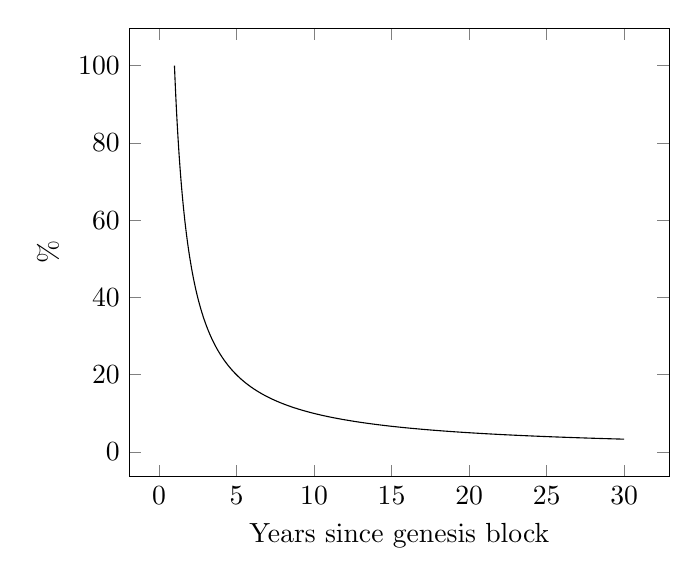
\begin{tikzpicture}
        \begin{axis}[
                xlabel = {Years since genesis block},
                ylabel = {\%},
            ]
            \addplot[
                domain=1:30,
                samples=1000,
            ]{100 * 1/x};
        \end{axis}
    \end{tikzpicture}
    \caption{Monetary inflation of mets}
    \label{fig:metinflation}
\end{figure}

Rewards to stakeholders come from two sources: met inflation and transaction fees. Stakeholders proposing new blocks earn rewards of 1 newly minted met per block, just like how Bitcoin miners earn a fixed per-block reward. This implicitly taxes unstaked mets, discourages holding mets without staking them. Since we mint a fixed amount of mets every block, the growth rate in the number of mets approaches zero. Figure \ref{fig:metinflation} illustrates the decreasing monetary inflation rate of mets.

Transaction fees, denominated in mels, are imposed on every transaction on the network. These fees also go entirely to the stakeholders as an additional source of income. The details of exactly how much transaction fees are charged and exactly how they are paid out to stakeholders are a little complicated, as Themelio uses a unique transaction fee model, different from that of other cryptocurrencies, in order to make it easier for clients to calculate appropriate fees. We discuss transaction fees in a separate document; for now a reasonable approximation is that stakeholders can extract most of the economic value generated by transactions as fees.

Slashing is the ``stick'' for punishing cryptographically provable misbehavior. The last step of our Byzantine-fault-tolerant consensus protocol has all stakeholders \emph{commit} to a particular block by signing it cryptographically. Honest stakeholders will always commit a valid block and never ``go back'' on its decision. Thus, we have two \emph{slashing conditions} which leave cryptographic proof that a certain stakeholder is dishonest:

\begin{itemize}
    \item \textbf{Equivocation}, where a stakeholder commits to two different blocks with the same block height
    \item \textbf{Invalid block}, where a stakeholder commits to an invalid block
\end{itemize}

In either of these cases, anybody can submit cryptographic evidence (two conflicting signatures, or a signature on an invalid block) as a specially-formatted transaction on the blockchain. This \textbf{slashing transaction} removes the offending stakeholder, deleting all of the lents associated with the stake. Slashing also reduces the supply of lents and increases the fraction of rewards that other stakeholders receive. This incentivizes large stakeholders to monitor each other and slash misbehaving stakeholders.

\subsubsection{Why two currencies?}

One of the unique features of Themelio's proof of stake is its separate staking token, the met, with features that intentionally discourage use as money. Generally, PoS blockchains use their main ``money'' coin, like ethers or EOS, as their staking asset. Why not do the same for Themelio? Coins used as stake for consensus are fundamentally equity shares. They are tokens representing fractional ownership of the transaction fees and other ``profit'' of the system. Unfortunately, \emph{equity shares are a poor form of money}.

First of all, for money we want flexible, demand-responsive monetary policies to reduce value volatility. Otherwise, the currency becomes an unpredictable store of value and a useless unit of account. In the offline world, this is accomplished either by central bank policies for fiat money, or natural supply elasticity for commodity money. For equity shares though, unpredictable share dilution demolishes their fundamental value proposition as fixed slices of profit. Thus, fixed minting schedules, like those of bitcoins and mets, are perfect for equity, but terrible for a new currency.

Furthermore, demand for equity shares in an efficient market is driven largely by speculation on future cash flow, while demand for cash derives from the need for a medium of exchange. We don't want users of a currency to be forced to speculate on the future transaction fees of a blockchain. Furthermore, increases in currency adoption as a means of exchange shouldn't drive destabilizing bubbles in currency value.

Themelio therefore uses an independent currency, the met, for the role of equity stake. This allows us to use an innovative, decentralized mechanism to stabilize the price of cels (discussed in \mytodo{TODO}) while keeping equity-like behavior for the ``investor'' token.

\subsubsection{Achieving high performance}

Scalable blockchains with immediate finality need a way to limit the number of consensus participants. This is because Byzantine fault-tolerant consensus algorithms have rapidly increasing overhead with increasing participants. To achieve our key design goal of scalability and performance, we are forced to limit the number of stakeholders to below a few thousand.

Themelio's way of restricting the number of stakeholders is through the minimum requirement of 1,000 mets staked per validator. Essentially, we limit entry into the oligarchy of stakeholders to only the richest met holders. Since met supply follows a fixed schedule, this places a hard limit of a few hundred new validators a year, so that growth in overhead won't outpace growth in computational capacity.

Although this is a very simple mechanism of restricting the number of consensus participants, it does not seem to be popular among existing proof-of-stake variants. We think this is most likely because a large minimum stake is politically unappealing. After all, it ``disenfranchises'' the vast majority of potential stakeholders and institutes a ``plutocracy''! Unfortunately, other approaches that superficially sound more decentralized tend to have crippling problems. Ironically, they end up a lot more vulnerable to centralized threats.

For example, a common method of deriving a small amount of participants from a large body of coinholders is \textit{delegated proof of stake} (DPoS). In DPoS, coinholders vote for people with voting power proportional to their coin ownership, and only the few with the most votes become ``delegates'' and participate in consensus. EOS is a popular blockchain using DPoS.

Yet although DPoS gives a vote to all coinholders, it insulates coinholders from protocol incentives. Coinholders are not responsible for the actions of the delegates they vote for, while misbehaving delegates receive no punishment other than a loss of reputation. Thus, coinholders have no incentive to vote for ``good'' nodes, delegates have little incentive to behave correctly, and misbehavior is rampant. Unsurprisingly, all the problems of political governance in a representative democracy get imported. Elections involve massive advertising campaigns, vote-buying, and even nationalist agitation \cite{zhihu2019votebuy}. Delegates routinely behave as a corrupted centralized cartel, engaging in actions like censoring transactions \mytodo{cite} and inflating the currency \mytodo{cite}.

\textit{Sortition} is another approach, used most notably in Algorand \cite{gilad2017algorand}. Periodically, a committee of participants is randomly selected from all coinholders --- each coinholder has a probability to win this ``lottery'' in proportion to the coins that they hold. The committee then participates in a consensus protocol to decide new blocks until the next lottery comes around.

Sortition eliminates most of the politics-like problems of DPoS, allowing protocol incentives like rewards and slashing to work fairly well. Unfortunately, severe problems remain. Randomly selecting participants trustlessly turns out to be a surprisingly hard cryptogrpahic problem --- a corrupt lottery can reliably elect malicious committees. Bribery attacks also become much easier, since instead of buying 1/3 of the coins, attackers can simply bribe the current committee, who has only a small fraction of the stake. Complex consensus protocols and advanced, non-quantum-resistant cryptographic techniques can reduce both challenges. But ``fancy'' mechanisms generally go against Themelio's philosophy of future-proof simplicity.

A point must be made that \textit{blockchain consensus is not analogous to political governance}. Themelio's ``plutocratic oligarchy'' of stakeholders certainly does not make for an effective way of electing a parliament. But for blockchains, it yields highly robust and decentralized security. It disperses control over blockchain consensus to the few hundred people most invested in the health of the network. At the same time, the protocol keeps them correctly behaving with massive carrots and sticks. Stakeholders do not decide political questions for the Themelio community; their only job is to run the consensus algorithm correctly.

Thus, we do not believe that Themelio's ``plutocratic'' bonded proof of stake is any more vulnerable to centralized threats than PoS blockchains without minimum stake amounts. Even so, Themelio has a system of \textit{auditors} keeping stakeholders in check, ensuring that even a fully corrupted quorum of stakeholders cannot do much damage.

\subsection{Auditors: the free press}

\subsubsection{Making failure catastrophic}

The ``free press'' in Themelio consists of \emph{auditors}. Auditors are ``full nodes'' in usual terminology, replicating and validating the entire blockchain. They form a random \emph{gossip} network among themselves, similar to that used by Bitcoin full nodes. Through this gossip network, information about new blocks is disseminated. Gossip reduces load on the stakeholders and makes it difficult for malicious networks to censor the blockchain --- as long as some auditors can connect to the stakeholders and the auditors form a connected graph, new blocks will quickly be visible to every auditor.

The more important role of auditors, though, is to \textit{make consensus failure catastrophic}. This plays a crucial role in keeping the oligarchy of stakeholders honest. Auditors utilize their position as relayers of new blocks to continually monitor for evidence that the stakeholder consensus is corrupt. For example, invalid blocks or two different blocks at the same height signed by a quorum would be proof that the coordinators are no longer trustworthy. These pieces of evidence, known as \textit{consensus nukes}, undeniably prove that at least 1/3 of the stakeholders are actively malicious or compromised.

Any auditor that sees a consensus nuke immediately broadcasts it to all auditors it knows in the gossip network. It then permanently activates a ``kill switch'' and refuses to operate normally. Thus, an attempt at forking or appending invalid transactions to the blockchain would figuratively "nuke" the entire network.

\subsubsection{Why consensus nukes?}

This objective seems a little strange. Why would we ever want our network to self-destruct?

The obvious answer is that if we no longer have a 2/3 supermajority of honest stake, the entire system is irrecoverable. More specifically, a well-known result \cite{dwork1988consensus} mathematically proves that consensus protocols running in a partially synchronous network model (that is, network delays are unknown but finite) cannot possibly tolerate more than 1/3 arbitrary faults. So we have to choose between a model where the network stays up, but malicious stakeholders can corrupt the state arbitrarily (rewriting history, giving themselves free money --- or shutting down the network), or one where the only thing a corrupted quorum can do is shut down the network. Clearly, the latter is preferable.

\marginpar{Consensus nuking can be seen as a variation on ``engineering security through coordination problems'', a concept explored in a blog post by Vitalik Buterin \cite{buterin2017coordination}, where attacks by cartels are made impractical because they would require coordinating many users to go along with them.}

More importantly, consensus nuking changes the incentives of potential attackers by making most attacks unprofitable. Consider a blockchain where consensus-breaking attacks (like Bitcoin's 51\% attack) allow arbitrary state corruption. A malicious actor with the ability to execute such attacks can extract huge profits simply through double-spending. With more complex higher-level applications relying on blockchain data, profit opportunities are even more numerous. Thus, if enough rationally self-serving stakeholders collude, they are greatly incentivized to attack the network and destroy its security guarantees.

If a successful attack can only result in the network stopping all work, only attackers who benefit from destroying the network will participate. Since a successful attacker must stake a vast amount of mets to take over more than 1/3 of the stake, destroying the network and thus the value of the investment is usually irrational.

Finally, a shutdown when a successful attack occurs forces Themelio users to manually coordinate an emergency ``hard fork'' out-of-band to restore the network. This would involve, at the very least, a redistribution of stakes away from the attacking parties and possibly protocol improvements to prevent future attacks. On the other hand, if the blockchain continues to operate even when stakeholders are corrupting the state, nothing forces users to coordinate a hard fork. It's conceivable that the malicious stakeholder cartel can create a climate of fear or pressure for users to go along with the corrupted chain --- for example, the state corruption might be forced by legal regulation or presented as way of restoring stolen assets. Consensus nuking ensures that these scenarios are impossible.

\subsection{Clients: thin yet fully secure}

Most users of a blockchain, Themelio not excepted, do not have nearly enough resources to process all transactions 24/7. Users that do not synchronize the whole blockchain state, known as thin clients, serve a vital role in any blockchain system. In other blockchains, though, thin clients come with both reduced security and mediocre performance. Bitcoin, for example, has thin clients who must persistently store a growing set of block headers and connect to at least one trusted full node.

In Themelio, thin clients (usually just called clients) are both thinner and safer than thin clients in other systems. Clients only synchronize a small piece of data, less than a kilobyte in size, a few times a year. Yet with this data, they can fully validate a large variety of information they can freely obtain from auditors. Even if a client only connects to bad auditors, it cannot be fooled into accepting invalid data. We accomplish this through two technical innovations: \textit{metastate commitments} in block headers and \textit{epoch-based stake bonds}.

\subsubsection{Metastate commitments}

Blocks in Themelio, like those in almost all blockchains, have constant-size \textit{headers} that summarize information about that block. Block headers typically cryptographically \textit{commit} to certain pieces of information, such as the transactions within a block, through hash trees and similar mechanisms. Cryptographic commitments allow thin clients to verify claims about the data they commit to without trusting third parties or downloading the entire blockchain.

In traditional coin-based blockchains, block headers commit only to the previous block header and the transactions within the block. This means thin clients can only verify claims that a certain transaction occurred in a block --- this is not enough even for basic applications like wallets to be trustless. Account-based blockchains like Ethereum improve on this by committing to the \textit{state}, or all the information needed to validate new transactions. This allows apps like wallets that rely on querying the state to run trustlessly.

In Themelio, the state is simply the set of all unspent coins. We use a sparse Merkle tree to commit in the block header to a mapping of the coin identifier (hash of the transaction that produced the coin and index of the coin) to coin metadata (value, constraint, etc). This allows thin clients to verify whether or not a coin is spent at a certain block height.

For some simple applications, like verifying a Catena log, this is sufficient. Unfortunately, many applications on coin-based blockchains need to access more than the plain state mapping. For example, wallets would want to know which coins to spend without proofs of payment from all incoming payers.

We therefore commit not just to the state mapping, but also to \textit{metastate}, or metadata about state. Metastate is not strictly necessary for validating blocks, but cryptographic commitments to it in the block header allows more powerful thin clients. This includes information like:
\begin{itemize}
    \item Number of unspent coins with a certain constraint
    \item Total number of transactions in the block
    \item Current block height
\end{itemize}

Thus, complex coin-oriented applications can trustlessly run on clients that don't need to synchronize anything but the latest block header.

\subsubsection{Epoch-based stake bonds}

One problem remains: how are clients supposed to get the latest block header? In many blockchains, clients simply synchronize \emph{all} the block headers. Clients would thus use ``proof-of-consensus'' information (in Bitcoin's case proof of work) embedded in each header to verify the next.

In Themelio, such a strategy would be prohibitively expensive. One of the tradeoffs we made that allows robust proof-of-stake immune to network problems is greatly increased sizes of proofs of consensus. A proof that a block header belongs to the valid blockchain in Themelio requires cryptographic signatures from at least 2/3 of the stakeholders --- about 10 KiB for a reasonable number of stakeholders. Furthermore, there are just a lot more blocks in Themelio than in Bitcoin. Instead of blocks 10 minutes apart, Themelio produces a block every 30 seconds. This means that in just a year, the block header consensus proofs would amount to more than 10 GB.

To fix this problem, Themelio divides blocks into \textit{epochs} lasting 500,000 blocks, or about half a year. Within each epoch, the list of shareholders and their respective voting weights stays the same. All stake-related transactions, such as staking and slashing, take effect only at the start of the next epoch. Finally, the last block header of each epoch embeds a \textit{stake document}, which includes the shareholders and voting weights to use when validating blocks in the next epoch.

This means that to validate, say, block header 1,100,000, we simply need the stake document embedded in block 999,999. And to validate that stake document, we just use the stake document in block 499,999. This process repeats until we get to a stake document we already know about.

So clients simply have to catch up on all the new stake documents they missed --- 10 KB every 6 months. Afterwards, they can securely validate the latest block header, which then lets them check claims about almost any fact about coins. Such ultra-thin clients allow apps using Themelio to scale on small devices like smartphones, while keeping trust totally decentralized.

\section{Cryptocurrency and economics}

Finally, we examine the cryptocurrency economy of Themelio, based on a low-volatility currency called the \textbf{mel}.

\subsection{Mels: low-volatility money}

Mels (TMEL) are optimized to be the day-to-day transaction currency on Themelio. One can imagine decentralized apps, grocery stores, and peer-to-peer finance to conduct transactions mainly denominated in TMEL.

The most important attribute of the mel is its \textit{low price volatility}. All mels are minted through a currency issuance algorithm we published called Elasticoin. With Elasticoin, we fix the \emph{cost} of minting new coins to 24 hours of provable sequential computation, instead of using the fixed \emph{schedule} of mining that Bitcoin or Ethereum uses.

A fixed minting cost makes supply highly elastic --- increases in mel price above cost will increase supply, while mels trading below cost will dry up the supply of new mels. Elasticoin has a rather elaborate mechanism to make sure that the minting cost does indeed track the cost of running sequential computation for a day, even as computers get faster.

Although simply fixing the cost to produce new mels will reduce its volatility drastically compared to fixed-schedule coins like Bitcoin, it's not completely sufficient for making the mel a useful currency. After all, it's conceivable nobody wants mels at all, making its price go to zero, and it wouldn't matter how much it costs to mint new mels since nobody even wants existing ones. Thus, we ensure that mels are always in demand by specifying that transaction fees must be paid in mels.

\subsection{Better transaction fees}

As in Bitcoin and other public blockchains, each transaction in Themelio includes a transaction fee to compensate stakeholders and make flooding attacks costly. Most other blockchains let transaction senders voluntarily decide whatever fee they like; block creators then decide which transactions to include in the limited space within a block. This functions as a pretty fair and efficient first-price auction, since transactions with more fees relative to the burden they pose to the network get higher priority. Unfortunately, auction-based transaction fees paid to whoever included the transaction in a block have several significant problems:

\begin{itemize}
    \item \textbf{Fees are extremely volatile}. When blocks are filled, average fees will vary quite a lot as demand fluctuates. In practice, persistently full blocks is the norm, whether due to demand increase in protocols like Bitcoin where the block size cap is fixed, or due to block producers setting block limits according to demand as in Ethereum. Thus, fees for full blocks are extremely volatile in existing blockchains, often changing as much as 2x within one block interval. This makes for a very poor user experience.
    \item \textbf{Complex client-side fee estimation}. It's far from trivial how much fees to bid in order to get transactions confirmed in a traditional fee market. Wallets need complicated algorithms to estimate the right amount of fee based on looking at unconfirmed transactions --- which thin clients can't even securely monitor.
    \item \textbf{Stakeholder incentive problems}. In a proof-of-stake system like Themelio, we want stakeholder income to come primarily from transaction fees. That way, stakes have values in proportion to the value of the system, making attacks harder as usage grows (and damage increases), while giving stakeholders a disincentive to collude to run Themelio into the ground. But a conventional fee market encourages stakeholders to hide transactions from each other --- a transaction you include in a block is a transaction fee that I didn't get --- leading to all sorts of pathological ``fee-stealing'' strategies unless stakeholders have a different source of income. This is why Bitcoin and Ethereum rely heavily on inflation, not fees, to reward block producers, but we don't want that in Themelio.
\end{itemize}

Thus, we abandon the traditional fee auction model in favor of a system inspired by EIP-1559. Every transaction pays a mel-denominated fee that has two components. A mandatory \textit{base fee} is calculated by multiplying by the \textit{base fee multiplier} the \textit{weight} of a transaction, a metric that roughly measures its cost. Transaction senders can then add a \textit{tip} above and beyond the base fee.

Every time a new block is created, the stakeholder proposing the block can adjust the base fee multiplier by up to 1\% upwards or downwards --- the base fee multiplier then reflects the stake-weighted median of the stakeholders' preferences. Base fees, except for an eighth which is burned, are deposited into a special \textit{fee pool} regardless of who included the transaction into the blockchain; the stakeholder creating a block then withdraws a tiny fraction ($1/65536$) of the fee pool. The net effect is that the base fee of a transaction is distributed to all stakeholders regardless of who made the block that contains the transaction.

Tips, on the other hand, are simply paid to the block producer, like fees in traditional blockchains. We expect tips to be a small fraction of total fees, and they give an incentive for block producers to actually include transactions instead of freeloading on a fee pool replenished by other, more honest block producers.

\begin{figure}
    \centering 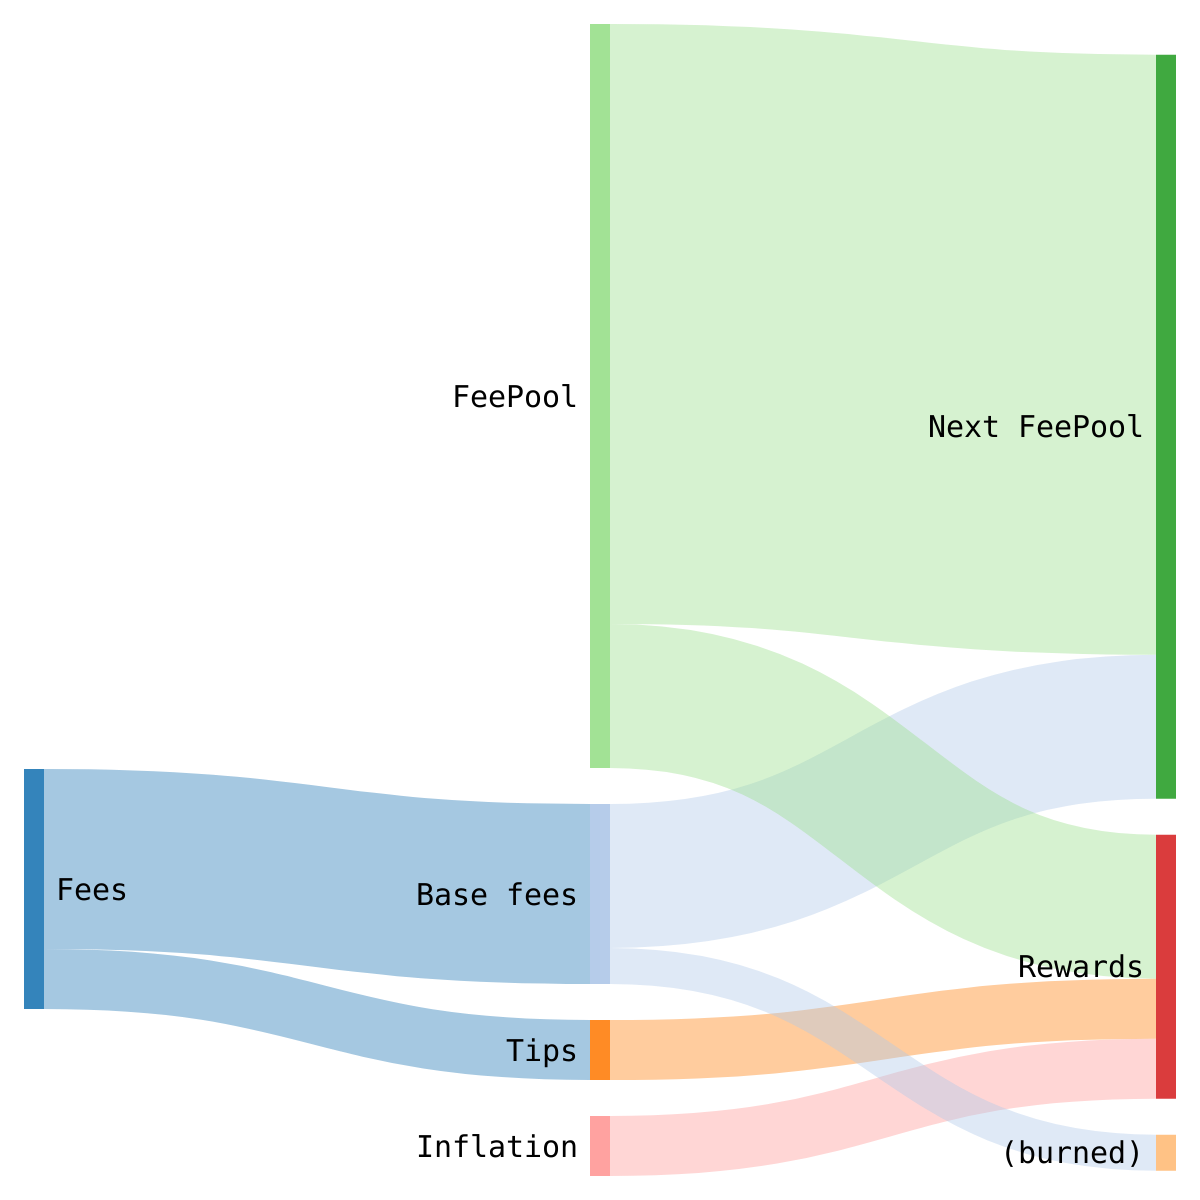
\includegraphics[width=0.7\linewidth]{fees.png}
    \caption{Per-block producer rewards (including met inflation)}
    \label{fig:fees}
\end{figure}

Figure \ref{fig:fees} illustrates the flow of funds every time a new block is created.

Why do our changes to the fee market fix its problems? First of all, fee volatility is greatly reduced. When demand fluctuates in the short term, it would be block sizes that fluctuate, not fees. Stakeholders adjust the base fee multiplier to maximize revenue and limit block sizes, but not rigidly at a defined size. One might object that stakeholders can collude to recreate Bitcoin's fee market --- by holding down the multiplier to zero, enforcing an unofficial block size limit, and auctioning off block space based on tips. But a rational stakeholder cartel will not do so, as assuming no change in demand, this will simply greatly increase income volatility without increasing expected total income, while in reality volatile fees will probably scare away some users, actually reducing revenue. Incidentally, this is also why we award base fees to stakeholders rather than burning them as in EIP-1559, since burning base fees will make colluding to create a fee aucion highly profitable.

Secondly, clients no longer need complex algorithms to compute fees. The base fee plus a small tip will be sufficient in all cases to get a transaction onto the blockchain as fast as possible. Applications like wallets or payment processors would easily predict the amount of fees needed.

Finally, although we still reward stakeholders with some met inflation to discourage passive met-holding, the use of a fee pool ensures that even though stakeholders are rewarded mostly from fees, there's no incentive to steal fees. In fact, one can think of the fee pool as a sort of long-term trust fund, derived from fees, for a stable Bitcoin-like block reward.

\chapter{Applications}

Finally, let's look at some possible applications on Themelio, and how they'd work. Unlike blockchains like Ethereum, it's not always straightforward to run an application directly on Themelio. Let's see, starting from simple to complicated apps, how with the help of certain upper-layer abstractions, decentralization be much more robust and performant.

\section{Scalable payment networks}

Obviously, on-chain mel transactions can be used directly to send money. However, as Themelio only processes at most 1000 transactions a second, this does not scale to the extent required for global microtransactions.

Fortunately, a solution already exists: payment channels. Payment channels, used in protocols like Lightning Network on Bitcoin or Raiden on Ethereum, allow secure cryptocurrency payments without either trusting third parties or conducting every transaction on the blockchain. Existing payment channel constructions for coin-based blockchains, like the Poon-Dryja channels used in Lightning Network, can easily be ported to Themelio. Perhaps more importantly, MelScript allows powerful bidirectional payment channels to be constructed in a straightforward manner without hacks such as the temporary keypairs used in Poon-Dryja channels.

Compared to payment channel networks on blockchains like Bitcoin or Ethereum, a Themelio PCN would provide far better scalability simply due to the faster blockchain --- after all, opening and closing payment channels is still limited by blockchain throughput. And compared to the traditional banking network, payment channels give immediate trustless finality, without any authorities that can steal funds or reverse payments. Even on the scalability side, a payment channel network on Themelio will greatly outperform traditional methods in volume and latency, allowing custodian-free microtransactions for applciations like paying road tolls.

\section{Decentralized naming}

Using blockchains to implement decentralized and secure naming systems is not a new use case. Blockstack, ENS, and Bitforest are all examples of blockchain-backed naming systems, which consistently map human-readable identifiers (such as domain names) to security-critical information like public keys without trusting third parties. Legacy naming systems, like DNS and CA-based PKI, are highly centralized and have very fragile security, so even for traditional centralized services like websites, a blockchain-backed, easily deployable naming system can significantly improve security.

Themelio's coin-based programming paradigm is especially suited for making naming systems. By using a \emph{coin index tree}, a data structure introduced by Bitforest, we can actually encode names as verifiable paths within the transaction DAG and map them to coins. Name transfers after the initial registration are simply transfers of this coin to new owners; more details can be found in the Bitforest paper.

Compared to existing blockchain solutions, a Themelio-based naming system would offer higher performance due to the blockchain's higher throughput, and more importantly, the ability for constant-space thin clients to quickly look up and verify names. Themelio's powerful thin-client abilities allow deploying blockchain-based naming directly to the smallest of edge devices, rather than relying on trusted gateways like in Blockstack. This removes one of the biggest challenges in deploying naming systems with fully decentralized trust.

\section{Token systems}

Another major use case for Themelio is for tokens, like fundraising tokens, cryptokitties, and new cryptocurrencies. Right now, a token is most commonly implemented as a big stateful smart contract on Ethereum, following API standards like ERC-20. This way of implementing a token, unfortunately, is prone to error, often leading to critical security vulnerabilities. Scalability is also a big challenge, as massive stateful smart contracts cannot be easily parallelized even with advanced features like sharding.

In Themelio, on the other hand, custom tokens are ridiculously easy to create. Themelio tokens rely on a special case in its transaction verification logic. Transactions must be balanced by currency --- the total values of mels, mets, etc in the input coins spent must be equal to the total values in the outputs --- with the exception that an unlimited number of coins, with unconstrained values, can be created with \textit{unlabeled} units. Outputs with unlabeled units will then create coins in the blockchain state with a new unit derived from the unique ID of the transaction.

Thus, a new cryptocurrency token can be created simply by creating any regular transaction while tacking on an additional unlabeled output with the value set to the maximum supply of the new token. This coin's constraint script will then determine the rules of token issuance --- no other transactions can create coins with the same unit, since custom tokens are always denominated by the first transaction that created them.

As an example, imagine Foobar wants to create a new token, FooCoin. FooCoin would be sold to the public at a fixed rate of 1000 nanomels per coin. Foobar would broadcast a transaction, say with ID \texttt{0xdeadbeef}, with an unlabeled output with an inexhaustibly large value (say $2^{64}$) and the following constraint:

\begin{lstlisting}
;; first output sends the rest of the FooCoins
;;   and repeats this constraint
;; second output sends FooCoin to buyer
;; third output sends mels to Foobar
(and (output-like? 0
      #:currency 0xdeadbeef
      #:constraint (output-constraint *SELF*))
     (output-like? 1
      #:currency 0xdeadbeef)
     (output-like? 2
      #:currency 'nTMEL
      #:constraint FOOBAR
      #:value (* (output-value (output-ref 0))
                  1000)))
\end{lstlisting}

Anybody can then spend this FooCoin-denominated output, diverting some of the FooCoin to himself, leaving the rest with the same constraint, and giving FooBar mels in compensation. FooCoins not encumbered by this constraint freely transact using the same rules as mets and mels do, with no complex smart contracts needed to handle all the cases. Wallet software, payment processors, etc can simply check for coins denominated in ``\texttt{0xdeadbeef}'' to support FooCoins.

Analogous constraints can be used to implement more complex rules for fungible cryptocurrency tokens. Non-fungible tokens are implemented simply by creating an a new token unit with a coin that has a value of 1. Since 1 cannot be further subdivided, this means that only one coin of that token can ever exist.  

\section{Secure computation}



\section{Public-consensus private blockchains}

\chapter{Conclusion}


\printbibliography

\end{document}
